% Copyright 2020 Glen Newton
% License: Creative Commons Attribution-ShareAlike 4.0 International License https://creativecommons.org/licenses/by-sa/4.0/legalcode

\documentclass{article}
\usepackage{tikz}
\usepackage[extreme]{savetrees}
\usepackage{microtype}
\usetikzlibrary{mindmap}

% from: https://tex.stackexchange.com/questions/250150/formatting-mindmap-in-tikz

\begin{document}
\sffamily
\pagestyle{empty}
          {\centering
            \makebox[0pt]{%
              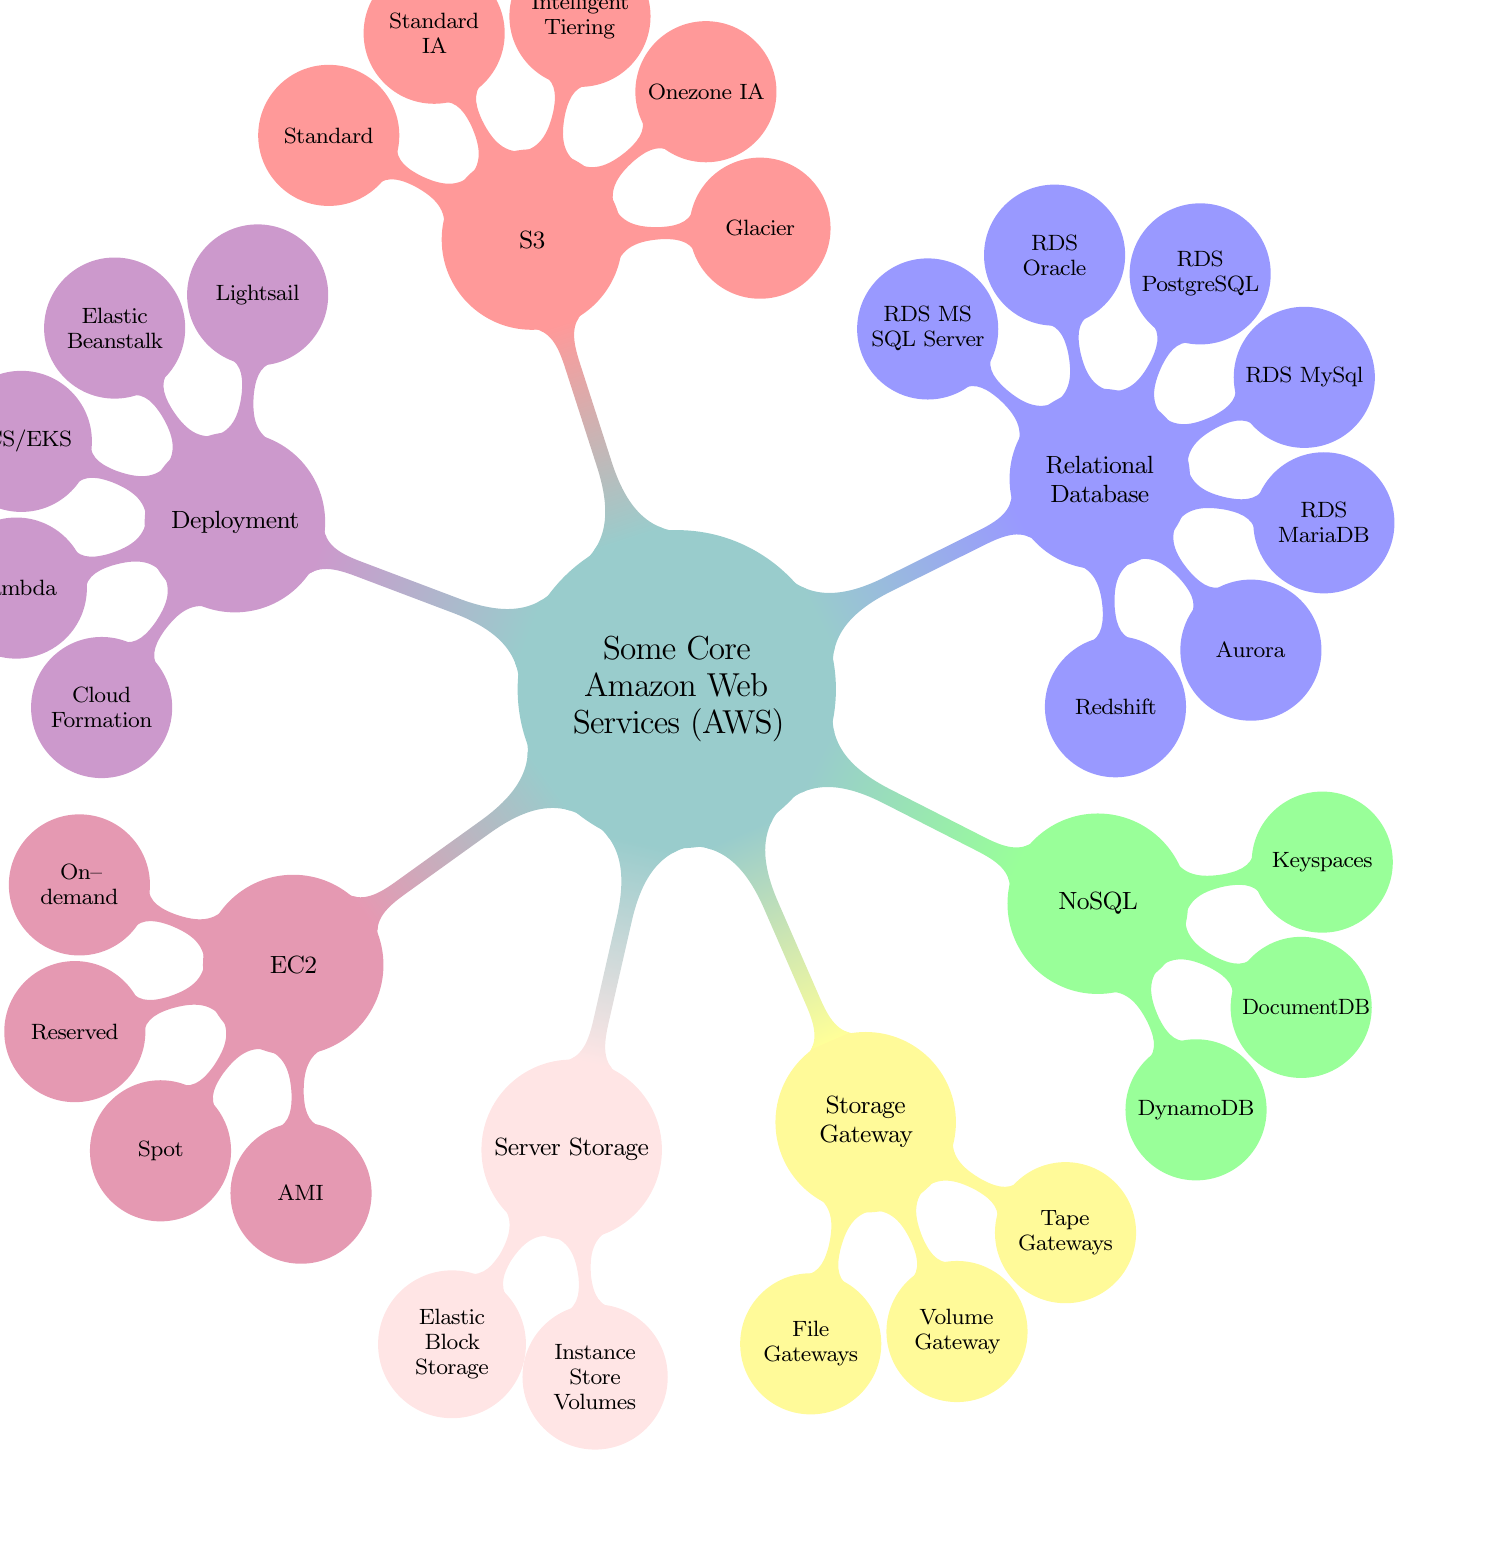
\begin{tikzpicture}
                [mindmap,
                  grow cyclic,
                  every node/.style=concept,
                  concept color=teal!40,
                  level 1/.append style={sibling angle=360/7, level distance=6cm},
                  level 2/.append style={sibling angle=37.5},
                ]
                \node [root concept] {Some Core Amazon Web Services (AWS)}
                child [concept color=purple!40, rotate=10]{
                  node    {EC2}
                  child { node    {On--demand} }
                  child { node    {Reserved} }
                  child { node    {Spot} }
                  child { node    {AMI} }
                }
                child [concept color=pink!40, rotate=0]{
                  node[concept] {Server Storage}
                  child { node[concept] {Elastic Block Storage} }
                  child { node[concept] {Instance Store Volumes} }
                }
                child [concept color=yellow!40, rotate=-15]{
                  node   {Storage Gateway}%[clockwise from=45, level distance=8cm]
                  child { node[concept] {File Gateways} }
                  child { node[concept] {Volume Gateway} }
                  child { node[concept] {Tape Gateways} }
                }
                child [concept color=green!40, rotate=-27]{
                  node     {NoSQL}
                  child { node    {DynamoDB } }
                  child { node    {DocumentDB} }
                  child { node    {Keyspaces} }
                }
                child [concept color=blue!40, rotate=-25]{
                  node     {Relational Database}
                  child { node[concept] {Redshift} }
                  child { node[concept] {Aurora} }
                  child { node[concept] {RDS MariaDB} }
                  child { node[concept] {RDS MySql} }
                  child { node[concept] {RDS PostgreSQL} }
                  child { node[concept] {RDS Oracle} }
                  child { node[concept] {RDS MS SQL Server} }
                }
                child [concept color=red!40, rotate=5]{node  {S3}[clockwise from=45]
                  child { node[concept] {Standard} }
                  child { node[concept] {Standard IA} }
                  child { node[concept] {Intelligent Tiering} }
                  child { node[concept] {Onezone IA} }
                  child { node[concept] {Glacier} }
                }
                child [concept color=violet!40, rotate=5] {
                  node {Deployment}
                  child { node {Lightsail} }
                  child { node {Elastic Beanstalk} }
                  child { node {ECS/EKS} }
                  child { node {Lambda} }
                  child { node {Cloud Formation} }
                };
            \end{tikzpicture}}\par}
\end{document}
